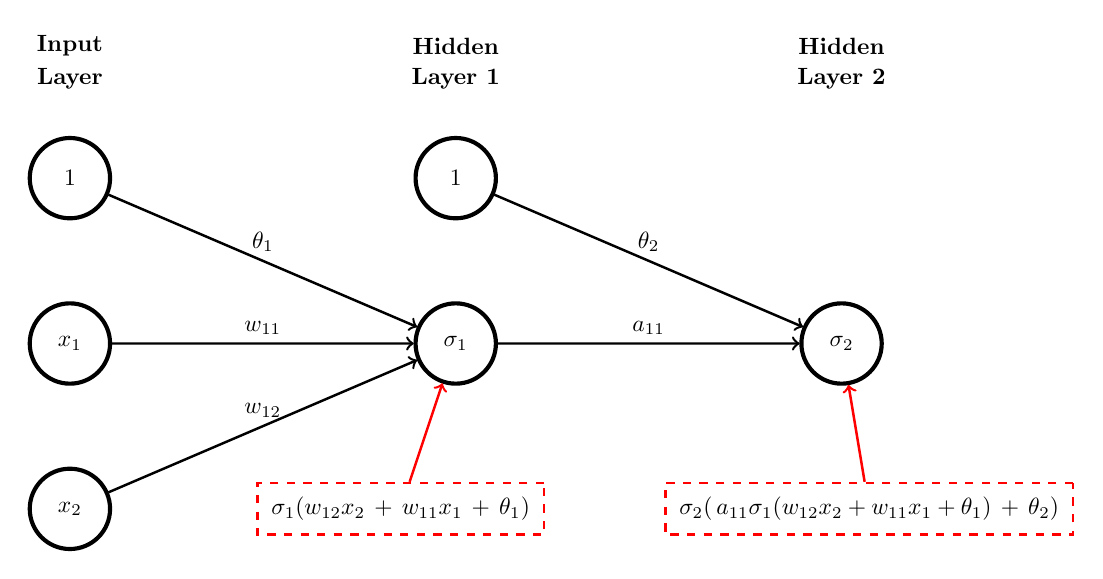
\begin{tikzpicture}[scale=0.7, every node/.style={scale=0.85}]

    %--------------------%
    % Parameters
    %--------------------%
    \def\layersep{7}
    \def\ysep{3}
    \def\circlesize{1.2cm}
    \def\shift{1}
    \def\woffset{5}
    \def\linethic{1.5pt}
    \def\arrowthic{0.6*\linethic}

    %--------------------%
    % Input Layer
    %--------------------%
    \node[draw, circle, minimum size=\circlesize, line width=\linethic] (theta1) at (0,2*\ysep) {1};
    \node[draw ,circle, minimum size=\circlesize, line width=\linethic] (x1) at (0,1*\ysep) {$x_1$};
    \node[draw ,circle, minimum size=\circlesize, line width=\linethic] (x2) at (0,0*\ysep) {$x_2$};

    %--------------------%
    % Layer 1
    %--------------------%
    % Nodes
    \node[draw, circle, minimum size=\circlesize, line width=\linethic] (theta2) at (\layersep,2*\ysep) {1};
    \node[draw ,circle, minimum size=\circlesize, line width=\linethic] (sigma1) at (\layersep,1*\ysep) {$\sigma_{1}$};
    \node[draw=red, rectangle, line width=1pt, dashed, fill=white, inner sep=6pt] (calc1) at (\layersep-\shift,0*\ysep) {$\sigma_{1}(w_{12} x_2 \,+\, w_{11} x_1 \,+\, \theta_1)$};
    

    %--------------------%
    % Layer 2
    %--------------------%
    \node[draw, circle, minimum size=\circlesize, line width=\linethic] (sigma2) at (2*\layersep,1*\ysep) {$\sigma_{2}$};
    
    \node[draw=red, rectangle, line width=1pt, dashed, fill=white, inner sep=6pt] (calc2) at (2*\layersep+0.5*\shift,0*\ysep) {$\sigma_{2}(\, a_{11} \sigma_{1}(w_{12} x_2 + w_{11} x_1 + \theta_1) \,+\, \theta_2)$};

    %--------------------%
    % Connections
    %--------------------%
    \draw[->, line width=\arrowthic] (theta1) -- node[above,midway]{$\theta_1$} (sigma1);
    \draw[->, line width=\arrowthic] (x1) -- node[above,midway]{$w_{11}$} (sigma1);
    \draw[->, line width=\arrowthic] (x2) -- node[above,midway]{$w_{12}$} (sigma1);
   
    \draw[->, line width=\arrowthic] (theta2) -- node[above,midway]{$\theta_2$} (sigma2);
    \draw[->, line width=\arrowthic] (sigma1) -- node[above,midway]{$a_{11}$} (sigma2);

    \draw[->, red, line width=\arrowthic] (calc1) -- node[above,midway]{} (sigma1);
    \draw[->, red, line width=\arrowthic] (calc2) -- node[above,midway]{} (sigma2);

    %--------------------%
    % Layer Labels
    %--------------------%
    \node at (0*\layersep, 2.8*\ysep) {\textbf{Input}};
    \node at (0*\layersep, 2.6*\ysep) {\textbf{Layer}};
    \node at (1*\layersep, 2.8*\ysep) {\textbf{Hidden}};
    \node at (1*\layersep, 2.6*\ysep) {\textbf{Layer 1}};
    \node at (2*\layersep, 2.8*\ysep) {\textbf{Hidden}};
    \node at (2*\layersep, 2.6*\ysep) {\textbf{Layer 2}};
\end{tikzpicture}
